\documentclass[A4paper]{article}
\usepackage[a4paper, total={7.2in, 10.5in}]{geometry}
\usepackage{tikz}
\usetikzlibrary{calc}
\usepackage{setspace}
\usepackage{graphicx}
\usepackage{amsmath}
\usepackage{pgfplots}
\usepackage[hidelinks]{hyperref}
\usepackage{bookmark}
\setcounter{tocdepth}{1}
\DeclareMathOperator\cosec{cosec}
\newcommand{\mycomment}[1]{}
\title{A Level Pure Mathematics Notes}
\author{Xingzhi Lu}
\date{For exam in 2025}

\usepackage{mathptmx}

\begin{document}
	\maketitle
	
	\section{Proof}
	\subsection{Methods}
	\begin{itemize}
		\item Proof by deduction
		\item Proof by exhaustion
		\item Disproof by counter example
		\item Proof by contradiction
	\end{itemize}
	\subsection{Proof by contradiction}
	\subsubsection{Steps}
	\begin{enumerate}
		\item Assume that the first statement is false
		\item Use logical steps / contradiction from knowledge to show that the assumption is false
		\item Conclude that the assumption is false so the original statement must be true
	\end{enumerate}
	\subsubsection{Irrationality of $\sqrt{2}$}
	\begin{description}
		\item [Assumption:] $\sqrt{2}$ is a rational number
		\item Then $\sqrt{2} = \dfrac{a}{b}$ for some integers $a$ and $b$
		\item Also assume that $a$ and $b$ has no common factors so the fraction is in the simplest form
		\item So $2=\dfrac{a^2}{b^2}$, $a^2=2b^2$
		\item So $a^2$ must be even, so a is also even
		\item If $a$ is even, then it can be expressed in the form $a=2n$, where $n$ is an integer
		\item Substitute $a=2n$: $(2n)^2=2b^2$
		\item So $4n^2 = 2b^2$
		\item So $b^2=2n^2$, hence $b^2$ must be even and b is also even
		\item If $a$ and $b$ are both even, they will have a common factor or 2
		\item This contradicts that $a$ and $b$ has no common factors, so $\sqrt{2}$ is an irrational number
	\end{description}


	\subsubsection{Infinity of primes}
	\begin{description}
		\item [Assumption:] there is a finite number of prime numbers
		\item List all the prime numbers that exist: $p_1, p_2, p_3, \dots, p_n$
		\item Consider the number $N = p_1 \times p_2 \times p_3 \times \dots \times p_n + 1$
		\item When $N$ is divided by any of $p_1, p_2, p_3, \dots, p_n$ a remainder of $1$ is produced so none of them is a factor of $N$
		\item Therefore $N$ must be prime or have a prime factor not in the list of all the prime numbers that exist
		\item This contradicts the assumption that there is a finite number of prime numbers
		\item Therefore there must be an infinite number of prime numbers
	\end{description}


	\pagebreak

	\section{Algebra and functions}
	
	\subsection{Indices}
	\begin{itemize}
		\item $a^m \times a^n = a^{m+n}$
		\item $a^m \div a^n = a^{m-n}$
		\item $(a^m)^n = a^{mn}$
		\item $a^{\frac{m}{n}} = \sqrt[n]{a^m}$
	\end{itemize}
	
	\subsection{Surds}
	\subsubsection{Rationalising the denominator}
	Multiply both the numerator and the denominator by the conjugate of the denominator
	
	\subsection{Expressing solutions with set notations}
	\subsubsection{Symbols}
	\begin{description}
		\item[And:] $\cap$
		\item[Or:] $\cup$
		\item[Greater than, smaller than, etc.:] $\left\lbrace x:x>k\right\rbrace$, $\left\lbrace x:x<k\right\rbrace$, etc.
		\item[Describing in words:] $x$ is such that $x$ is greater / less than / greater than or equal to / less than or equal to $k$ and $x$ is a real number
	\end{description}
	\subsubsection{Examples}
	\begin{itemize}
		\item $x>a$ and $x<b$ can be expressed as $\left\lbrace x : x>a \right\rbrace \cap \left\lbrace x:x<b\right\rbrace$
		\item $x<c$ or $x>d$ can be expressed as $\left\lbrace x : x>c \right\rbrace \cup \left\lbrace x:x<d\right\rbrace$
	\end{itemize}

	\subsection{Sketching graphs}
	\subsubsection{Quadratic / cubic / quartic}
	Find:
	\begin{itemize}
		\item Roots (may only be one or none)
		\item y-intercept
		\item Turning point
		\item Shape
	\end{itemize}

	\subsubsection{Reciprocal graphs}
	Find:
	\begin{itemize}
		\item Horizontal asymptotes (by long division)
		\item Vertical asymptotes (where denominator = $0$)
	\end{itemize}


	\pagebreak

	\section{Coordinate geometry in $(x,y)$ plane}
	
	\subsection{Straight line graphs}
	\subsubsection{Finding equation of graphs}
	$\dfrac{y-y_1}{y_2-y_1}=\dfrac{x-x_1}{x_2-x_1}$
	
	\subsubsection[]{*Distance from a point to a line}
	$d=\dfrac{|ax_0+by_0+c|}{\sqrt{a^2+b^2}}$\\
	
	\subsection{Modelling with linear equations}
	\subsubsection{Commenting on validity for very large / small values}
	Think about:
	\begin{enumerate}
		\item The range of values that the data has (is it including very large / small values?)
		\item What may happen as value becomes very small / large (is it realistic?)
	\end{enumerate}

	\subsection{Parametric equations}
	\subsubsection{Convert to Cartesian form}
	\begin{itemize}
		\item Express $t$ in terms of $x$, then substitute $t=f(x)$ into $y=g(t)$
		\item Find the range of $x$ by using the original parametric equation
		\item Find the range of $y$ using original equation / considering the domain of $x$
	\end{itemize}
	\subsubsection{Sketching curves}
	Sketch at regular intervals of $t$


	\pagebreak

	\section{Sequences and series}
	\subsection{Binomial expansion}
	* Always write the answer in \textbf{ascending} powers of $x$
	\subsubsection{Expanding $(1+x)^n$}
	When $|x|<1$:\\
	$(1+x)^n\approx 1 + nx + \dfrac{n(n-1)}{2!}x^2+\dfrac{n(n-1)(n-2)}{3!}x^3+\dots$
	\subsubsection{Expanding $(a+bx)^n$}
	$(a+bx)^n = (a(1+\dfrac{b}{a}x))^n = a^n(1+\dfrac{b}{a}x)^n$\\
	Valid for $|\dfrac{b}{a}x|<1$ or $|x| < \dfrac{a}{b}$
	\subsection{Divergent / convergent series}
	$\sum\limits_{i=1}^{n} u_i = u_1+u_2+u_3+\dots+u_n$\\
	If $\lim\limits_{n \to \infty}S_n$ exists, $\sum\limits_{i=1}^{n} u_i$ converges\\
	If $\lim\limits_{n \to \infty}S_n$ does not exist, $\sum\limits_{i=1}^{n} u_i$ diverges
	\subsection{Geometric series}
	\begin{description}
		\item [Sum of first n terms:]$S_n = \dfrac{a(1-r^n)}{1-r}$
		\item [Sum to infinity:] When $|r|<1$ (convergent series): $S_\infty = \dfrac{a}{1-r}$
	\end{description}

	\subsection{Recurrence relations}
	\begin{description}
		\item[Increasing sequence:] $u_{n+1}>u_n$ for all $n\in \mathbf{N}$
		\item[Decreasing sequence:] $u_{n+1}<u_n$ for all $n\in \mathbf{N}$
		\item[Periodic sequence:] If there is an integer $k$ such that $u_{n+k}=u_n$ for all $n\in \mathbf{N}$, $k$ = the order of the sequence
	\end{description}

	\pagebreak

	\section{Trigonometry}
	\subsection{Radian calculations}
	\begin{description}
		\item[Arc length:] $s=r\theta$
		\item[Area of sector:] $A=\dfrac{1}{2}r^2\theta$
	\end{description}

	\subsection{Trigonometry formulae}
	\subsubsection{Addition / subtraction}
	\begin{itemize}
		\item $\sin (A \pm B) = \sin A \cos B \pm \cos A \sin B$
		\item $\cos (A \pm B) = \cos A \cos B \mp \sin A \sin B$
		\item $\tan (A \pm B) = \dfrac{\tan A \pm \tan B}{1 \mp \tan A \tan B}$
	\end{itemize}
	\subsubsection{Sum to product identities}
	\begin{itemize}
		\item $\sin A + \sin B = 2\sin \dfrac{A+B}{2} \cos\dfrac{A-B}{2}$
		\item $\sin A - \sin B = 2\cos \dfrac{A+B}{2} \sin\dfrac{A-B}{2}$
		\item $\cos A + \cos B = 2\cos \dfrac{A+B}{2} \cos\dfrac{A-B}{2}$
		\item $\cos A - \cos B = -2\sin \dfrac{A+B}{2} \sin\dfrac{A-B}{2}$
	\end{itemize}
	\subsubsection{Double angle}
	\begin{itemize}
		\item $\sin 2A = 2\sin A \cos A$
		\item $\cos 2A = \cos^2 A - \sin^2 A$
		\item $\tan 2A = \dfrac{2\tan A}{1-\tan^2 A}$
	\end{itemize}
	\subsubsection{Power descending}
	(Derive from double angle)
	\begin{itemize}
		\item $\sin A \cos A = \dfrac{\sin2A}{2}$
		\item $\sin^2 A = \dfrac{1-\cos2A}{2}$
		\item $\cos^2 A = \dfrac{1+\cos2A}{2}$
	\end{itemize}
	\subsubsection{Half angle}
	\begin{itemize}
		\item $\sin \dfrac{A}{2} = \pm \sqrt{\dfrac{1-\cos A}{2}}$
		\item $\cos \dfrac{A}{2} = \pm \sqrt{\dfrac{1+\cos A}{2}}$
		\item $\tan \dfrac{A}{2} = \pm \sqrt{\dfrac{1-\cos A}{1+\cos A}} = \dfrac{1-\cos A}{\sin A} = \dfrac{\sin A}{1+\cos A}$
	\end{itemize}
	\subsubsection{Small angle estimation}
	When $\theta$ is small:
	\begin{itemize}
		\item $\sin \theta \approx \theta$
		\item $\cos \theta \approx 1- \dfrac{\theta^2}{2}$
		\item $\tan \theta \approx \theta$
	\end{itemize}
	\subsection{Identities}
	\begin{itemize}
		\item $\tan \theta = \dfrac{\sin \theta}{\cos \theta}$
		\item $\sin^2 \theta + \cos^2 \theta = 1$
		\item $\tan^2 \theta + 1 = \sec^2 \theta$
		\item $\cot^2 \theta + 1 = \cosec^2 \theta$
	\end{itemize}

	\subsection{Graphs}
	\subsubsection{secant, cosecant and cotangent}
	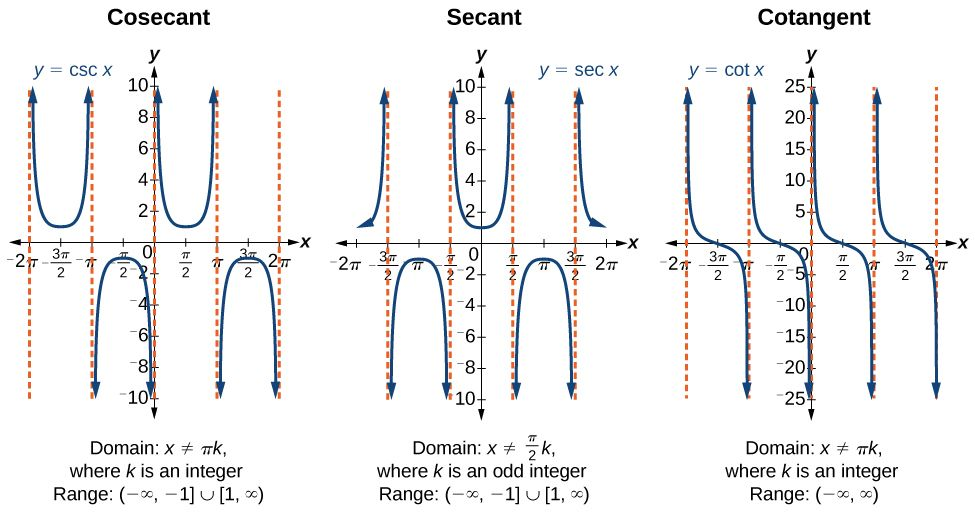
\includegraphics[scale=0.9]{csc-sec-cot-graphs}

	\subsubsection{arcsin, arccos, arctan}
	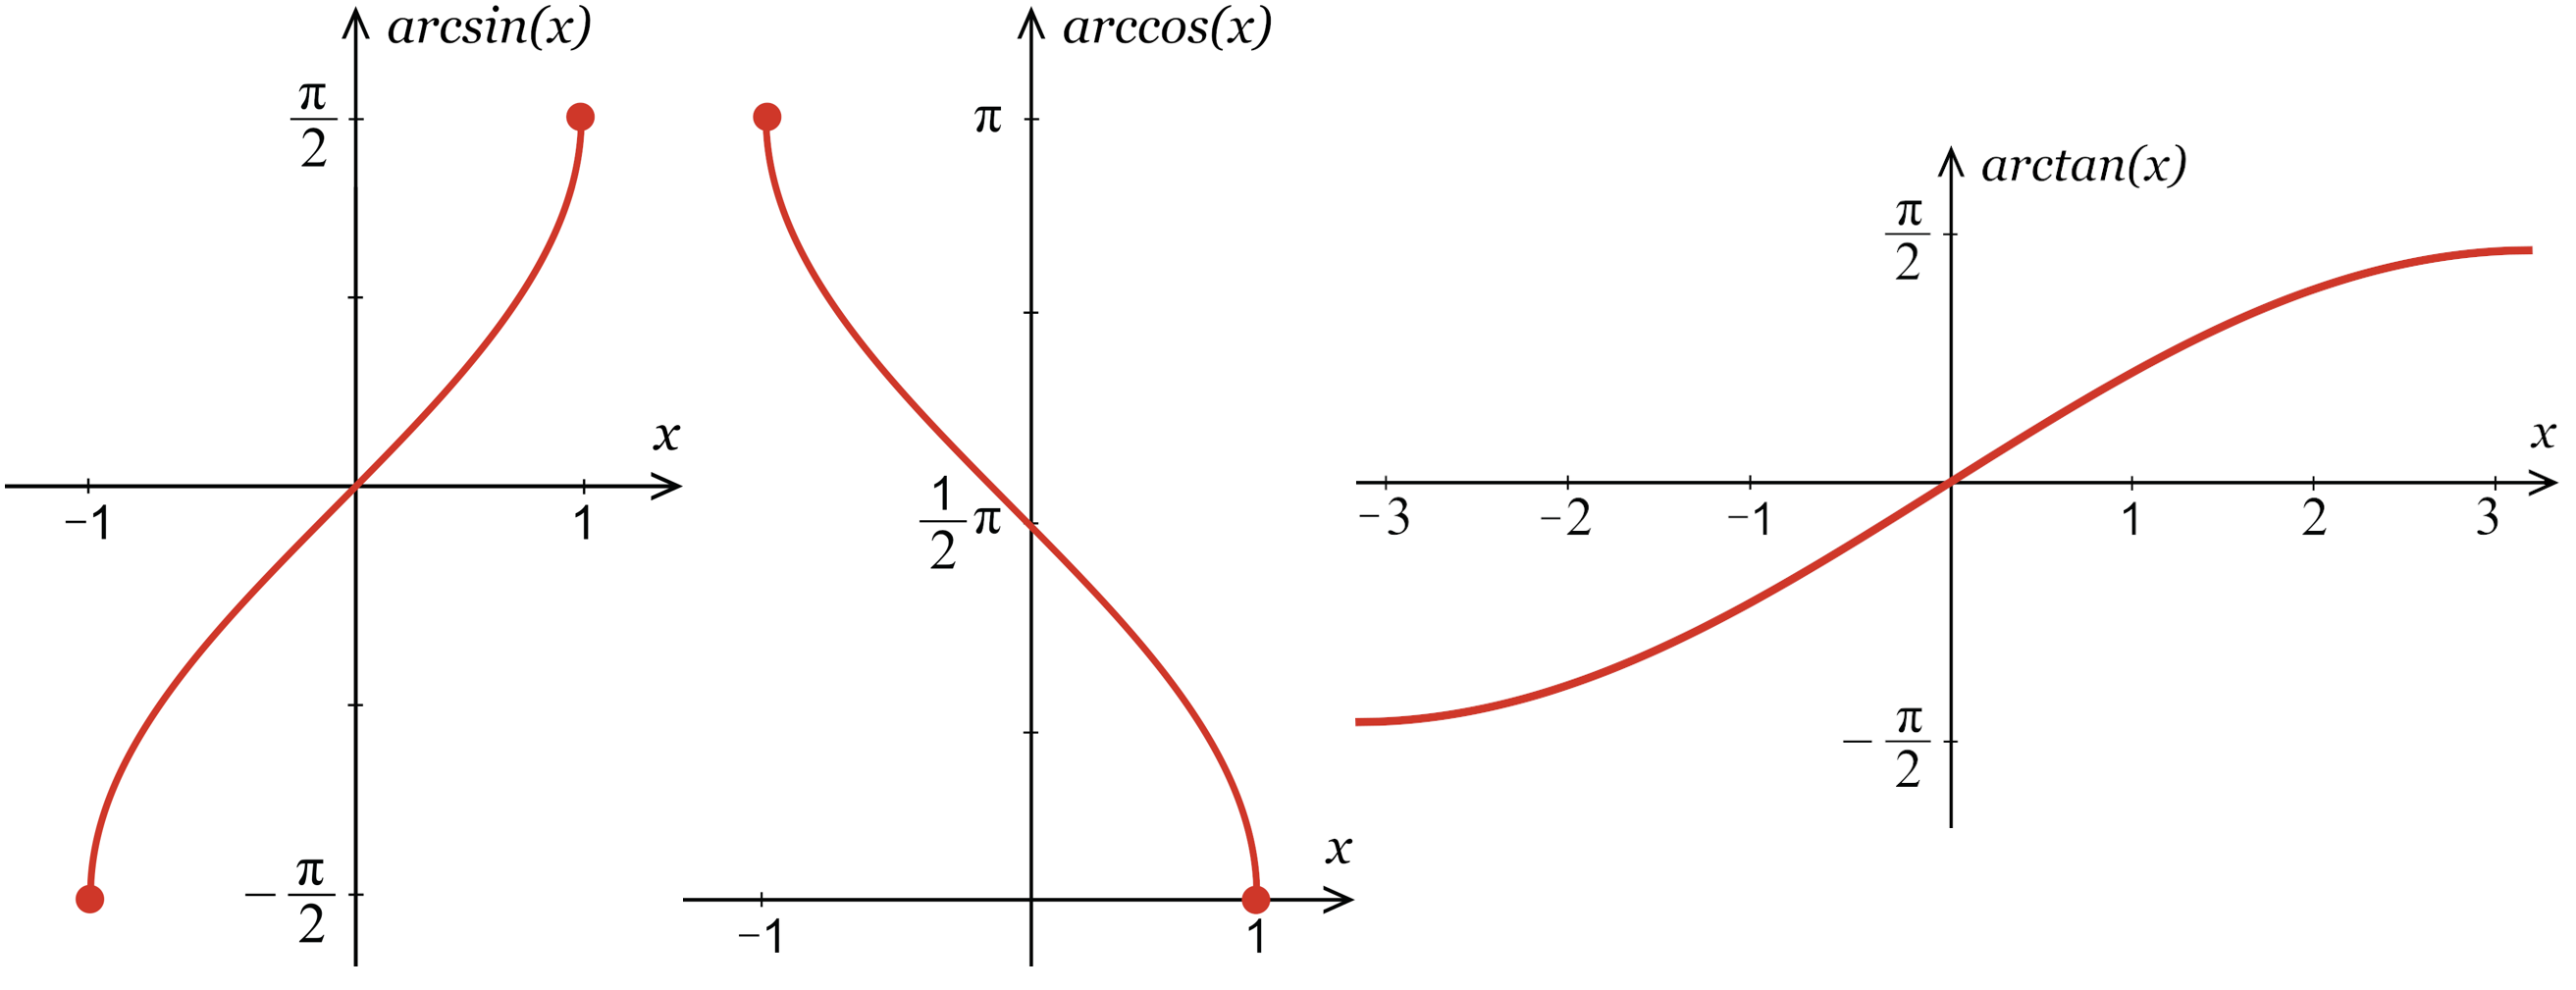
\includegraphics[scale=0.7]{arcsincostan}
	
	\subsection{Trig equations}
	\subsubsection{Principal values}
	The angle that you get when you use the inverse trigonometric functions on the calculator
	\begin{itemize}
		\item $\sin^{-1}$: $-90\leq\theta\leq90$
		\item $\cos^{-1}$: $0\leq\theta\leq180$
		\item $\tan^{-1}$: $-90\leq\theta\leq90$
	\end{itemize}
	
	\pagebreak

	\section{Exponentials and logarithms}
	\subsection{Sketching graphs}
	Find the y-intercept of the graph

	\subsection{$e^x$ function}
	\begin{description}
		\item $(e^x)'$ = $e^x$ (gradient = $y$ value)
		\item $(e^{kx})'$ = $ke^{kx}$ (gradient directly proportional to $y$ value)
	\end{description}

	\subsection{Logarithm}
	$a^x = n$: $\log_a n = x$ ($a\neq1$ and $a>0$, $x>0$)
	\subsubsection{Laws}
	\begin{description}
		\item[The multiplication law:] $\log_a x + \log_a y = \log_a xy$
		\item[The division law:] $\log_a x - \log_a y = \log_a (\dfrac{x}{y})$
		\item[The power law:] $\log_a x^k = k\log_a x$
		\item[Change base formula]: $\log_a b = \dfrac{\log_c b}{\log_c a}$
	\end{description}

	\subsubsection{Logarithms in non-linear form}
	\textbf{Exponential}
	\begin{itemize}
		\item $y=ab^x\rightarrow\ln y = x\ln b + \ln a$
		\item x-axis = $x$, y-axis = $\ln y$, gradient = $\ln b$, y-intercept = $\ln a$
	\end{itemize}
	\textbf{Power}
	\begin{itemize}
		\item $y=ax^b\rightarrow\ln y = b\ln x + \ln a$
		\item x-axis = $\ln x$, y-axis = $\ln y$, gradient = $b$, y-intercept = $\ln a$
	\end{itemize}
	\textbf{Logarithmic}
	\begin{itemize}
		\item $y=a\ln x\rightarrow$ kept the same
		\item x-axis = $\ln x$, y-axis = $y$, gradient = $a$
	\end{itemize}

	\pagebreak

	\section{Differentiation}

	$f'(x) = \lim\limits_{n \to 0}\dfrac{f(x+h)-f(x)}{h}$

	\subsection{Formulae}
	\begin{tabular}{ll}
		$\mathbf{f(x)}$ & $\mathbf{f'(x)}$ \\
		$\tan kx$ & $k\sec^2 kx$ \\
		$\sec kx$ & $k\sec kx \tan kx$ \\
		$\cot kx$ & $-k\cosec^2 kx$ \\
		$\cosec kx$ & $-k\cosec kx \cot kx$ \\
	\end{tabular}

	\subsection{Rules}
	\begin{description}
		\item[Chain rule:] $\dfrac{dy}{dx} = \dfrac{dy}{du} \times \dfrac{du}{dx}$
		\item[Product rule:] $(f(x)g(x))'=f'(x)g(x)+g'(x)f(x)$
		\item[Quotient rule:] $\dfrac{f(x)}{g(x)} = \dfrac{f'(x)g(x)-g'(x)f(x)}{g^2(x)}$
	\end{description}


	\subsection{Tangent and normal}
	For curve $y=f(x)$:
	\begin{description}
		\item[Tangent at $(a,f(a))$:] $y-f(a)=f'(a)(x-a)$
		\item[Normal at $(a,f(a))$:] $y-f(a)=-\dfrac{1}{f'(a)}(x-a)$
	\end{description}




	\pagebreak

	\section{Integration}
	
	\subsection{Definition}
	$\int_{a}^{b} f(x) \: dx = \lim\limits_{\delta x\rightarrow0}\sum_{x=a}^{b}f(x)\delta x$
	
	\subsection{Formulae}
	Formula sheet:\\\\
	\begin{tabular}{ll}
	$\textbf{f(x)}$	& \textbf{$\int f(x) \: dx$ ($+c$)} \\&\\ 
	$\sec^2kx$	& $\dfrac{1}{k} \tan kx$ \\&\\
	$\tan kx$	& $\dfrac{1}{k} \ln |\sec kx|$ \\&\\
	$\cot kx$	& $\dfrac{1}{k} \ln |\sin kx|$ \\&\\
	$\cosec kx$	& $-\dfrac{1}{k} \ln |\cosec kx + \cot kx|$, $\dfrac{1}{k} \ln |\tan (\dfrac{1}{2}kx)|$ \\&\\
	$\sec kx$	& $\dfrac{1}{k} \ln |\sec kx + \tan kx|$, $\dfrac{1}{k} \ln |\tan (\dfrac{1}{2}kx+\dfrac{1}{4}\pi)|$ \\

	\end{tabular}\\
	Integrating $\sin^2x$ or $\cos^2x$ (power descending):
	\begin{itemize}
		\item $\int \sin ^2 x \: dx=\int \dfrac{1-\cos 2x}{2} \: dx=\dfrac{1}{2}(x-\dfrac{\sin 2x}{2})+c$
		\item $\int \cos ^2 x \: dx=\int \dfrac{1+\cos 2x}{2} \: dx= \dfrac{1}{2}(x+\dfrac{\sin 2x}{2})+c$
	\end{itemize}
	By part:
	\begin{itemize}
		\item $\int \ln x \: dx = x\ln x + x + c$
	\end{itemize}
	\subsection{Techniques}
	\subsubsection{U-sub}
	\begin{itemize}
		\item $\int f'(ax+b) \: dx = \dfrac{f(ax+b)}{a}+c$
		\begin{description}
			\item[Substitution:] $u=ax+b$
		\end{description}
		\item $\int \dfrac{f'(x)}{f(x)} \: dx = \ln |f(x)|+c$
		\begin{description}
			\item[Substitution:] $u=f(x)$
		\end{description}
	\end{itemize}
	\subsubsection{By part}
	\begin{itemize}
		\item $\int u \: dv = uv - \int v \: du$
		\item LIPET rule: leftmost = $u$
		\begin{description}
			\item[L:] logarithmic
			\item[I:] inverse trigonometry
			\item[P:] polynomial
			\item[E:] exponential
			\item[T:] trigonometry
		\end{description}
	\end{itemize}
	
	
	\pagebreak

	\section{Numerical methods}
	\subsection{Locating roots}
	\subsubsection{Method}
	If a function $f(x)$ is continuous on the interval $[a,b]$ and $f(a)$ and $f(b)$ have opposite signs, then $f(x)$ has at least one root, $x$, which satisfies $a<x<b$
	\subsubsection{How change of sign can fail}
	\begin{itemize}
		\item When the interval is too large sign may not change as there may be an even number of roots
		\item If the function is not continuous, sign may change but there may be an asymptote e.g. reciprocal
	\end{itemize}
	
	\subsection{Iteration}
	\begin{itemize}
		\item Iterative formula can be found by rewriting $f(x)=0$ into $x=g(x)$, then $x_{n+1}=g(x_n)$
		\item Find the value of $x_1$, $x_2$, $x_3$, etc.
		\item If converge (get closer to the root from the same direction / alternate above and below the root) then solution can be found
		\item Test for roots using the change of sign of function $h(x)=g(x)-x$
	\end{itemize}
	
	\subsection{The Newton-Raphson method}
	\begin{itemize}
		\item $x_{n+1}=x_n-\dfrac{f(x_n)}{f'(x_n)}$
		\item Find approximation to $x$ decimal places
		\item Show accurate to $x$ decimal places: use change in sign to show
		\item[$\star$] If any value of $x_i$ is at a turning point then the method will fail as $f'(x)=0$ which results in division by zero
	\end{itemize}
	
	\subsection{The trapezium rule}
	$\int_{a}^{b}y\:dx \approx \dfrac{1}{2} h (y_0+2(y_1+y_2+\dots+y_{n-1})+y_n)$ where $h=\dfrac{b-a}{n}$ and $y_i=f(a+ih)$


	\pagebreak

	\section{Vectors}
	\subsection{Angle with x-, y-, and z-axis (direction cosines)}
	If $\vec{a}=x\vec{i}+y\vec{j}+z\vec{k}$ makes an angle $\theta_x$ with the positive x-axis then $\cos \theta_x=\dfrac{x}{|a|}$, similarly for angles $\theta_y$ and $\theta_z$
	\subsection{Vectors in equations}
	\subsubsection{2D}
	If $\vec{a}$ and $\vec{b}$ are 2 non-parallel vectors and $p\vec{a}+q\vec{b}=r\vec{a}+s\vec{b}$ then $p=r$ and $q=s$
	\subsubsection{3D}
	If $\vec{a}$, $\vec{b}$ and $\vec{c}$ are vectors in 3 dimensions which do not all lie on the same plane (parallel to the same plane) then you can compare their coefficients on both sides of an equation
	
	\subsection{Modelling with vectors}
	$\star$ Be careful about whether the question asked to use vector or scalar quantities
	\subsubsection{Vector quantities}
	\begin{itemize}
		\item $\vec{v}$ = velocity
		\item $\overrightarrow{AB}$ = displacement from $A$ to $B$
	\end{itemize}
	
	\subsubsection{Scalar quantities}
	\begin{itemize}
		\item $|\vec{v}|$ = speed
		\item $|\overrightarrow{AB}|$ = distance in a straight line from $A$ to $B$
	\end{itemize}
	
	
	
	
	\end{document}